%%%%%%%%%%%%%%%%%%%%%%%%%%%%%%%%%%%%%%%%%%
\section{Tracking}
\frame{\frametitle{Kalman Filter}

Obiettivo: stimare lo stato $x \in \Re^n$ di un processo a tempo discreto governato dalla seguente equazione alle differenze
\begin{equation*}
 x_k=Ax_{k-1}+Bu_{k-1}+w_{k-1}
\end{equation*}  


 L'osservazione (al tempo $k$) dello stato reale $x_k$ è effettuata tramite il vettore della misura $z \in \Re^m$ 


\begin{equation*}
z_k=Hx_k+v_k
\end{equation*}

\begin{figure}[hb]
\centering
	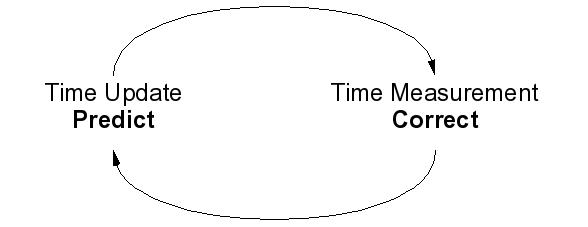
\includegraphics[scale=0.25]{../relazione/figure/PredCorr.jpg}
\caption{\textit{Il ciclio di calcolo del filtro di Kalman.}}
\end{figure}}
%%%%%%%%%%%%%%%%%%%%%%%%%%%%%%%%%%%%%%%%%%
